\documentclass[1p]{elsarticle_modified}
%\bibliographystyle{elsarticle-num}

%\usepackage[colorlinks]{hyperref}
%\usepackage{abbrmath_seonhwa} %\Abb, \Ascr, \Acal ,\Abf, \Afrak
\usepackage{amsfonts}
\usepackage{amssymb}
\usepackage{amsmath}
\usepackage{amsthm}
\usepackage{scalefnt}
\usepackage{amsbsy}
\usepackage{kotex}
\usepackage{caption}
\usepackage{subfig}
\usepackage{color}
\usepackage{graphicx}
\usepackage{xcolor} %% white, black, red, green, blue, cyan, magenta, yellow
\usepackage{float}
\usepackage{setspace}
\usepackage{hyperref}

\usepackage{tikz}
\usetikzlibrary{arrows}

\usepackage{multirow}
\usepackage{array} % fixed length table
\usepackage{hhline}

%%%%%%%%%%%%%%%%%%%%%
\makeatletter
\renewcommand*\env@matrix[1][\arraystretch]{%
	\edef\arraystretch{#1}%
	\hskip -\arraycolsep
	\let\@ifnextchar\new@ifnextchar
	\array{*\c@MaxMatrixCols c}}
\makeatother %https://tex.stackexchange.com/questions/14071/how-can-i-increase-the-line-spacing-in-a-matrix
%%%%%%%%%%%%%%%

\usepackage[normalem]{ulem}

\newcommand{\msout}[1]{\ifmmode\text{\sout{\ensuremath{#1}}}\else\sout{#1}\fi}
%SOURCE: \msout is \stkout macro in https://tex.stackexchange.com/questions/20609/strikeout-in-math-mode

\newcommand{\cancel}[1]{
	\ifmmode
	{\color{red}\msout{#1}}
	\else
	{\color{red}\sout{#1}}
	\fi
}

\newcommand{\add}[1]{
	{\color{blue}\uwave{#1}}
}

\newcommand{\replace}[2]{
	\ifmmode
	{\color{red}\msout{#1}}{\color{blue}\uwave{#2}}
	\else
	{\color{red}\sout{#1}}{\color{blue}\uwave{#2}}
	\fi
}

\newcommand{\Sol}{\mathcal{S}} %segment
\newcommand{\D}{D} %diagram
\newcommand{\A}{\mathcal{A}} %arc


%%%%%%%%%%%%%%%%%%%%%%%%%%%%%5 test

\def\sl{\operatorname{\textup{SL}}(2,\Cbb)}
\def\psl{\operatorname{\textup{PSL}}(2,\Cbb)}
\def\quan{\mkern 1mu \triangleright \mkern 1mu}

\theoremstyle{definition}
\newtheorem{thm}{Theorem}[section]
\newtheorem{prop}[thm]{Proposition}
\newtheorem{lem}[thm]{Lemma}
\newtheorem{ques}[thm]{Question}
\newtheorem{cor}[thm]{Corollary}
\newtheorem{defn}[thm]{Definition}
\newtheorem{exam}[thm]{Example}
\newtheorem{rmk}[thm]{Remark}
\newtheorem{alg}[thm]{Algorithm}

\newcommand{\I}{\sqrt{-1}}
\begin{document}

%\begin{frontmatter}
%
%\title{Boundary parabolic representations of knots up to 8 crossings}
%
%%% Group authors per affiliation:
%\author{Yunhi Cho} 
%\address{Department of Mathematics, University of Seoul, Seoul, Korea}
%\ead{yhcho@uos.ac.kr}
%
%
%\author{Seonhwa Kim} %\fnref{s_kim}}
%\address{Center for Geometry and Physics, Institute for Basic Science, Pohang, 37673, Korea}
%\ead{ryeona17@ibs.re.kr}
%
%\author{Hyuk Kim}
%\address{Department of Mathematical Sciences, Seoul National University, Seoul 08826, Korea}
%\ead{hyukkim@snu.ac.kr}
%
%\author{Seokbeom Yoon}
%\address{Department of Mathematical Sciences, Seoul National University, Seoul, 08826,  Korea}
%\ead{sbyoon15@snu.ac.kr}
%
%\begin{abstract}
%We find all boundary parabolic representation of knots up to 8 crossings.
%
%\end{abstract}
%\begin{keyword}
%    \MSC[2010] 57M25 
%\end{keyword}
%
%\end{frontmatter}

%\linenumbers
%\tableofcontents
%
\newcommand\colored[1]{\textcolor{white}{\rule[-0.35ex]{0.8em}{1.4ex}}\kern-0.8em\color{red} #1}%
%\newcommand\colored[1]{\textcolor{white}{ #1}\kern-2.17ex	\textcolor{white}{ #1}\kern-1.81ex	\textcolor{white}{ #1}\kern-2.15ex\color{red}#1	}

{\Large $\underline{12a_{0161}~(K12a_{0161})}$}

\setlength{\tabcolsep}{10pt}
\renewcommand{\arraystretch}{1.6}
\vspace{1cm}\begin{tabular}{m{100pt}>{\centering\arraybackslash}m{274pt}}
\multirow{5}{120pt}{
	\centering
	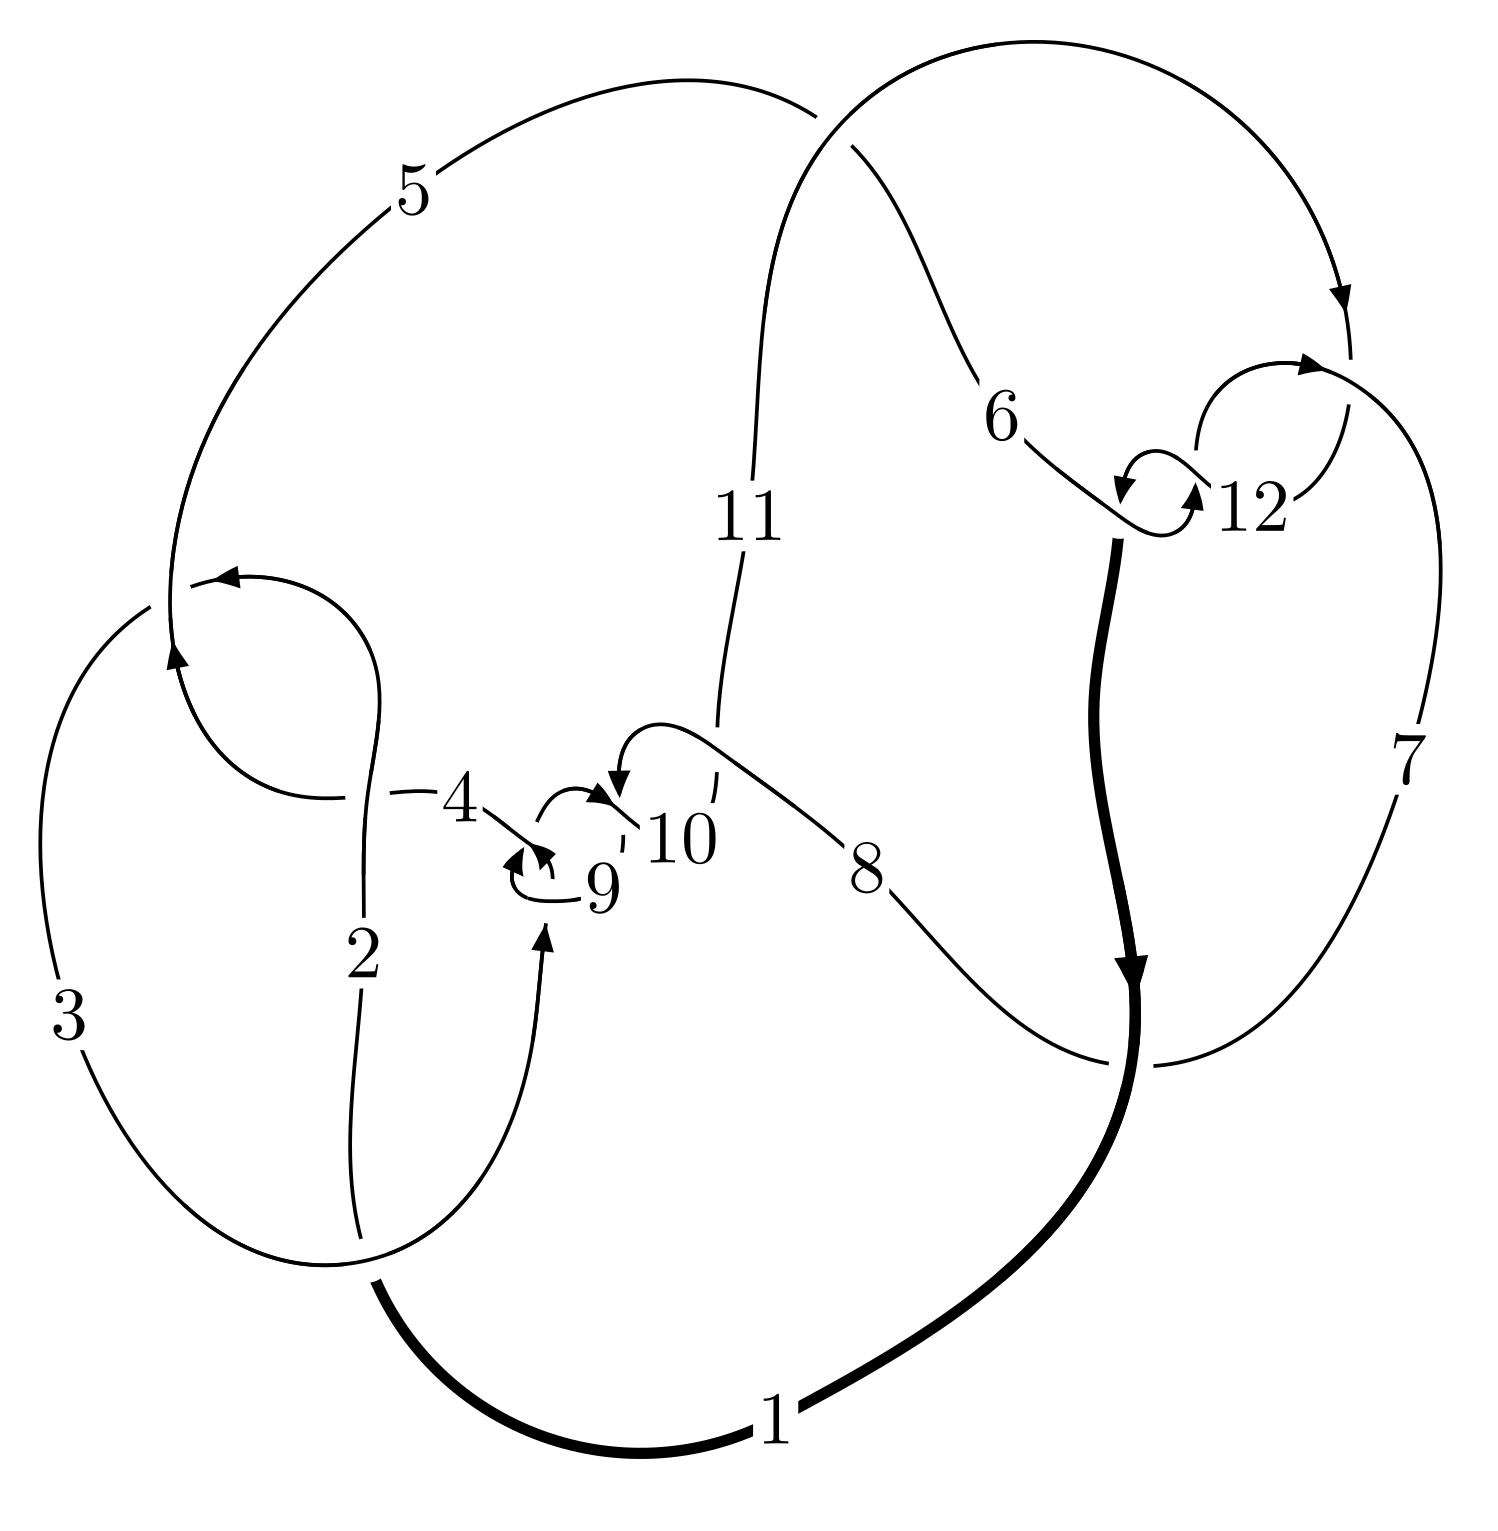
\includegraphics[width=112pt]{../../../GIT/diagram.site/Diagrams/png/962_12a_0161.png}\\
\ \ \ A knot diagram\footnotemark}&
\allowdisplaybreaks
\textbf{Linearized knot diagam} \\
\cline{2-2}
 &
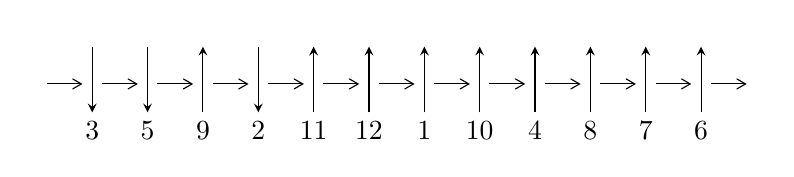
\begin{tikzpicture}[x=20pt, y=17pt]
	% nodes
	\node (C0) at (0, 0) {};
	\node (C1) at (1, 0) {};
	\node (C1U) at (1, +1) {};
	\node (C1D) at (1, -1) {3};

	\node (C2) at (2, 0) {};
	\node (C2U) at (2, +1) {};
	\node (C2D) at (2, -1) {5};

	\node (C3) at (3, 0) {};
	\node (C3U) at (3, +1) {};
	\node (C3D) at (3, -1) {9};

	\node (C4) at (4, 0) {};
	\node (C4U) at (4, +1) {};
	\node (C4D) at (4, -1) {2};

	\node (C5) at (5, 0) {};
	\node (C5U) at (5, +1) {};
	\node (C5D) at (5, -1) {11};

	\node (C6) at (6, 0) {};
	\node (C6U) at (6, +1) {};
	\node (C6D) at (6, -1) {12};

	\node (C7) at (7, 0) {};
	\node (C7U) at (7, +1) {};
	\node (C7D) at (7, -1) {1};

	\node (C8) at (8, 0) {};
	\node (C8U) at (8, +1) {};
	\node (C8D) at (8, -1) {10};

	\node (C9) at (9, 0) {};
	\node (C9U) at (9, +1) {};
	\node (C9D) at (9, -1) {4};

	\node (C10) at (10, 0) {};
	\node (C10U) at (10, +1) {};
	\node (C10D) at (10, -1) {8};

	\node (C11) at (11, 0) {};
	\node (C11U) at (11, +1) {};
	\node (C11D) at (11, -1) {7};

	\node (C12) at (12, 0) {};
	\node (C12U) at (12, +1) {};
	\node (C12D) at (12, -1) {6};
	\node (C13) at (13, 0) {};

	% arrows
	\draw[->,>={angle 60}]
	(C0) edge (C1) (C1) edge (C2) (C2) edge (C3) (C3) edge (C4) (C4) edge (C5) (C5) edge (C6) (C6) edge (C7) (C7) edge (C8) (C8) edge (C9) (C9) edge (C10) (C10) edge (C11) (C11) edge (C12) (C12) edge (C13) ;	\draw[->,>=stealth]
	(C1U) edge (C1D) (C2U) edge (C2D) (C3D) edge (C3U) (C4U) edge (C4D) (C5D) edge (C5U) (C6D) edge (C6U) (C7D) edge (C7U) (C8D) edge (C8U) (C9D) edge (C9U) (C10D) edge (C10U) (C11D) edge (C11U) (C12D) edge (C12U) ;
	\end{tikzpicture} \\
\hhline{~~} \\& 
\textbf{Solving Sequence} \\ \cline{2-2} 
 &
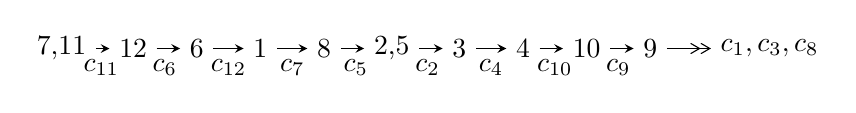
\begin{tikzpicture}[x=23pt, y=7pt]
	% node
	\node (A0) at (-1/8, 0) {7,11};
	\node (A1) at (1, 0) {12};
	\node (A2) at (2, 0) {6};
	\node (A3) at (3, 0) {1};
	\node (A4) at (4, 0) {8};
	\node (A5) at (81/16, 0) {2,5};
	\node (A6) at (49/8, 0) {3};
	\node (A7) at (57/8, 0) {4};
	\node (A8) at (65/8, 0) {10};
	\node (A9) at (73/8, 0) {9};
	\node (C1) at (1/2, -1) {$c_{11}$};
	\node (C2) at (3/2, -1) {$c_{6}$};
	\node (C3) at (5/2, -1) {$c_{12}$};
	\node (C4) at (7/2, -1) {$c_{7}$};
	\node (C5) at (9/2, -1) {$c_{5}$};
	\node (C6) at (45/8, -1) {$c_{2}$};
	\node (C7) at (53/8, -1) {$c_{4}$};
	\node (C8) at (61/8, -1) {$c_{10}$};
	\node (C9) at (69/8, -1) {$c_{9}$};
	\node (A10) at (11, 0) {$c_{1},c_{3},c_{8}$};

	% edge
	\draw[->,>=stealth]	
	(A0) edge (A1) (A1) edge (A2) (A2) edge (A3) (A3) edge (A4) (A4) edge (A5) (A5) edge (A6) (A6) edge (A7) (A7) edge (A8) (A8) edge (A9) ;
	\draw[->>,>={angle 60}]	
	(A9) edge (A10);
\end{tikzpicture} \\ 

\end{tabular} \\

\footnotetext{
The image of knot diagram is generated by the software ``\textbf{Draw programme}" developed by Andrew Bartholomew(\url{http://www.layer8.co.uk/maths/draw/index.htm\#Running-draw}), where we modified some parts for our purpose(\url{https://github.com/CATsTAILs/LinksPainter}).
}\phantom \\ \newline 
\centering \textbf{Ideals for irreducible components\footnotemark of $X_{\text{par}}$} 
 
\begin{align*}
I^u_{1}&=\langle 
- u^{45}-19 u^{43}+\cdots+b- u,\;u^{77}+u^{76}+\cdots+a-1,\;u^{78}+2 u^{77}+\cdots-4 u^2-1\rangle \\
I^u_{2}&=\langle 
u^2+b- u+1,\;-2 u^2+a-2,\;u^3- u^2+2 u-1\rangle \\
\\
\end{align*}
\raggedright * 2 irreducible components of $\dim_{\mathbb{C}}=0$, with total 81 representations.\\
\footnotetext{All coefficients of polynomials are rational numbers. But the coefficients are sometimes approximated in decimal forms when there is not enough margin.}
\newpage
\renewcommand{\arraystretch}{1}
\centering \section*{I. $I^u_{1}= \langle - u^{45}-19 u^{43}+\cdots+b- u,\;u^{77}+u^{76}+\cdots+a-1,\;u^{78}+2 u^{77}+\cdots-4 u^2-1 \rangle$}
\flushleft \textbf{(i) Arc colorings}\\
\begin{tabular}{m{7pt} m{180pt} m{7pt} m{180pt} }
\flushright $a_{7}=$&$\begin{pmatrix}0\\u\end{pmatrix}$ \\
\flushright $a_{11}=$&$\begin{pmatrix}1\\0\end{pmatrix}$ \\
\flushright $a_{12}=$&$\begin{pmatrix}1\\- u^2\end{pmatrix}$ \\
\flushright $a_{6}=$&$\begin{pmatrix}- u\\u^3+u\end{pmatrix}$ \\
\flushright $a_{1}=$&$\begin{pmatrix}u^2+1\\- u^4-2 u^2\end{pmatrix}$ \\
\flushright $a_{8}=$&$\begin{pmatrix}u^5+2 u^3+u\\- u^7-3 u^5-2 u^3+u\end{pmatrix}$ \\
\flushright $a_{2}=$&$\begin{pmatrix}- u^{77}- u^{76}+\cdots+4 u+1\\u^{45}+19 u^{43}+\cdots-8 u^2+u\end{pmatrix}$ \\
\flushright $a_{5}=$&$\begin{pmatrix}- u^3-2 u\\u^3+u\end{pmatrix}$ \\
\flushright $a_{3}=$&$\begin{pmatrix}- u^{51}-22 u^{49}+\cdots-16 u^2+6 u\\- u^{77}-2 u^{76}+\cdots-2 u^2+1\end{pmatrix}$ \\
\flushright $a_{4}=$&$\begin{pmatrix}2 u^{77}+2 u^{76}+\cdots-4 u-1\\- u^{77}-2 u^{76}+\cdots- u+1\end{pmatrix}$ \\
\flushright $a_{10}=$&$\begin{pmatrix}- u^{12}-5 u^{10}-9 u^8-6 u^6+u^2+1\\u^{14}+6 u^{12}+13 u^{10}+10 u^8-2 u^6-4 u^4+u^2\end{pmatrix}$ \\
\flushright $a_{9}=$&$\begin{pmatrix}u^{19}+8 u^{17}+26 u^{15}+42 u^{13}+31 u^{11}+2 u^9-10 u^7-4 u^5+u^3+2 u\\- u^{21}-9 u^{19}+\cdots- u^3+u\end{pmatrix}$\\&\end{tabular}
\flushleft \textbf{(ii) Obstruction class $= -1$}\\~\\
\flushleft \textbf{(iii) Cusp Shapes $= - u^{77}-2 u^{76}+\cdots+19 u+1$}\\~\\
\newpage\renewcommand{\arraystretch}{1}
\flushleft \textbf{(iv) u-Polynomials at the component}\newline \\
\begin{tabular}{m{50pt}|m{274pt}}
Crossings & \hspace{64pt}u-Polynomials at each crossing \\
\hline $$\begin{aligned}c_{1}\end{aligned}$$&$\begin{aligned}
&u^{78}+44 u^{77}+\cdots+17 u+1
\end{aligned}$\\
\hline $$\begin{aligned}c_{2},c_{4}\end{aligned}$$&$\begin{aligned}
&u^{78}-4 u^{77}+\cdots+9 u-1
\end{aligned}$\\
\hline $$\begin{aligned}c_{3},c_{9}\end{aligned}$$&$\begin{aligned}
&u^{78}- u^{77}+\cdots+4 u+8
\end{aligned}$\\
\hline $$\begin{aligned}c_{5},c_{7}\end{aligned}$$&$\begin{aligned}
&u^{78}-2 u^{77}+\cdots+4 u-1
\end{aligned}$\\
\hline $$\begin{aligned}c_{6},c_{11},c_{12}\end{aligned}$$&$\begin{aligned}
&u^{78}+2 u^{77}+\cdots-4 u^2-1
\end{aligned}$\\
\hline $$\begin{aligned}c_{8},c_{10}\end{aligned}$$&$\begin{aligned}
&u^{78}-21 u^{77}+\cdots-1232 u+64
\end{aligned}$\\
\hline
\end{tabular}\\~\\
\newpage\renewcommand{\arraystretch}{1}
\flushleft \textbf{(v) Riley Polynomials at the component}\newline \\
\begin{tabular}{m{50pt}|m{274pt}}
Crossings & \hspace{64pt}Riley Polynomials at each crossing \\
\hline $$\begin{aligned}c_{1}\end{aligned}$$&$\begin{aligned}
&y^{78}-16 y^{77}+\cdots-329 y+1
\end{aligned}$\\
\hline $$\begin{aligned}c_{2},c_{4}\end{aligned}$$&$\begin{aligned}
&y^{78}-44 y^{77}+\cdots-17 y+1
\end{aligned}$\\
\hline $$\begin{aligned}c_{3},c_{9}\end{aligned}$$&$\begin{aligned}
&y^{78}-21 y^{77}+\cdots-1232 y+64
\end{aligned}$\\
\hline $$\begin{aligned}c_{5},c_{7}\end{aligned}$$&$\begin{aligned}
&y^{78}-38 y^{77}+\cdots+8 y+1
\end{aligned}$\\
\hline $$\begin{aligned}c_{6},c_{11},c_{12}\end{aligned}$$&$\begin{aligned}
&y^{78}+66 y^{77}+\cdots+8 y+1
\end{aligned}$\\
\hline $$\begin{aligned}c_{8},c_{10}\end{aligned}$$&$\begin{aligned}
&y^{78}+67 y^{77}+\cdots-68864 y+4096
\end{aligned}$\\
\hline
\end{tabular}\\~\\
\newpage\flushleft \textbf{(vi) Complex Volumes and Cusp Shapes}
$$\begin{array}{c|c|c}  
\text{Solutions to }I^u_{1}& \I (\text{vol} + \sqrt{-1}CS) & \text{Cusp shape}\\
 \hline 
\begin{aligned}
u &= \phantom{-}0.221840 + 0.947945 I \\
a &= -0.90854 - 2.19426 I \\
b &= -0.63575 + 1.79124 I\end{aligned}
 & -6.03562 - 1.43380 I & \phantom{-0.000000 } 0 \\ \hline\begin{aligned}
u &= \phantom{-}0.221840 - 0.947945 I \\
a &= -0.90854 + 2.19426 I \\
b &= -0.63575 - 1.79124 I\end{aligned}
 & -6.03562 + 1.43380 I & \phantom{-0.000000 } 0 \\ \hline\begin{aligned}
u &= -0.322913 + 0.983251 I \\
a &= -0.59097 + 2.36662 I \\
b &= -0.89380 - 1.94580 I\end{aligned}
 & -5.23022 + 7.49440 I & \phantom{-0.000000 } 0 \\ \hline\begin{aligned}
u &= -0.322913 - 0.983251 I \\
a &= -0.59097 - 2.36662 I \\
b &= -0.89380 + 1.94580 I\end{aligned}
 & -5.23022 - 7.49440 I & \phantom{-0.000000 } 0 \\ \hline\begin{aligned}
u &= -0.266822 + 1.014570 I \\
a &= -0.265621 - 0.087182 I \\
b &= \phantom{-}0.763129 - 0.052329 I\end{aligned}
 & -2.10877 + 2.64422 I & \phantom{-0.000000 } 0 \\ \hline\begin{aligned}
u &= -0.266822 - 1.014570 I \\
a &= -0.265621 + 0.087182 I \\
b &= \phantom{-}0.763129 + 0.052329 I\end{aligned}
 & -2.10877 - 2.64422 I & \phantom{-0.000000 } 0 \\ \hline\begin{aligned}
u &= -0.201285 + 0.867169 I \\
a &= -0.61079 - 1.89983 I \\
b &= \phantom{-}0.17550 + 1.40684 I\end{aligned}
 & -6.10936 - 1.32608 I & \phantom{-}0.73693 + 1.24858 I \\ \hline\begin{aligned}
u &= -0.201285 - 0.867169 I \\
a &= -0.61079 + 1.89983 I \\
b &= \phantom{-}0.17550 - 1.40684 I\end{aligned}
 & -6.10936 + 1.32608 I & \phantom{-}0.73693 - 1.24858 I \\ \hline\begin{aligned}
u &= \phantom{-}0.316364 + 0.786903 I \\
a &= -0.12641 + 1.88878 I \\
b &= \phantom{-}0.12525 - 1.63413 I\end{aligned}
 & -5.61969 + 7.17353 I & \phantom{-}1.91318 - 7.13043 I \\ \hline\begin{aligned}
u &= \phantom{-}0.316364 - 0.786903 I \\
a &= -0.12641 - 1.88878 I \\
b &= \phantom{-}0.12525 + 1.63413 I\end{aligned}
 & -5.61969 - 7.17353 I & \phantom{-}1.91318 + 7.13043 I\\
 \hline 
 \end{array}$$\newpage$$\begin{array}{c|c|c}  
\text{Solutions to }I^u_{1}& \I (\text{vol} + \sqrt{-1}CS) & \text{Cusp shape}\\
 \hline 
\begin{aligned}
u &= -0.785147 + 0.185065 I \\
a &= -3.20268 + 3.17739 I \\
b &= \phantom{-}1.37992 - 2.53027 I\end{aligned}
 & -2.75716 - 11.61650 I & \phantom{-}5.77587 + 8.60798 I \\ \hline\begin{aligned}
u &= -0.785147 - 0.185065 I \\
a &= -3.20268 - 3.17739 I \\
b &= \phantom{-}1.37992 + 2.53027 I\end{aligned}
 & -2.75716 + 11.61650 I & \phantom{-}5.77587 - 8.60798 I \\ \hline\begin{aligned}
u &= -0.770791 + 0.171159 I \\
a &= \phantom{-}0.857137 + 0.494336 I \\
b &= -0.743484 + 0.108436 I\end{aligned}
 & \phantom{-}0.46016 - 6.59193 I & \phantom{-}9.04398 + 5.71613 I \\ \hline\begin{aligned}
u &= -0.770791 - 0.171159 I \\
a &= \phantom{-}0.857137 - 0.494336 I \\
b &= -0.743484 - 0.108436 I\end{aligned}
 & \phantom{-}0.46016 + 6.59193 I & \phantom{-}9.04398 - 5.71613 I \\ \hline\begin{aligned}
u &= \phantom{-}0.216613 + 0.756610 I \\
a &= -0.036625 + 0.331435 I \\
b &= \phantom{-}0.702068 - 0.142190 I\end{aligned}
 & -2.39928 + 2.61834 I & \phantom{-}4.76572 - 3.85328 I \\ \hline\begin{aligned}
u &= \phantom{-}0.216613 - 0.756610 I \\
a &= -0.036625 - 0.331435 I \\
b &= \phantom{-}0.702068 + 0.142190 I\end{aligned}
 & -2.39928 - 2.61834 I & \phantom{-}4.76572 + 3.85328 I \\ \hline\begin{aligned}
u &= -0.782132 + 0.079591 I \\
a &= -1.50273 + 2.21168 I \\
b &= \phantom{-}0.47522 - 1.74253 I\end{aligned}
 & \phantom{-}4.89842 - 5.92763 I & \phantom{-}11.50709 + 7.07473 I \\ \hline\begin{aligned}
u &= -0.782132 - 0.079591 I \\
a &= -1.50273 - 2.21168 I \\
b &= \phantom{-}0.47522 + 1.74253 I\end{aligned}
 & \phantom{-}4.89842 + 5.92763 I & \phantom{-}11.50709 - 7.07473 I \\ \hline\begin{aligned}
u &= -0.320177 + 1.177210 I \\
a &= -0.373766 + 1.202460 I \\
b &= -0.73975 - 1.50874 I\end{aligned}
 & \phantom{-}1.55633 + 1.91915 I & \phantom{-0.000000 } 0 \\ \hline\begin{aligned}
u &= -0.320177 - 1.177210 I \\
a &= -0.373766 - 1.202460 I \\
b &= -0.73975 + 1.50874 I\end{aligned}
 & \phantom{-}1.55633 - 1.91915 I & \phantom{-0.000000 } 0\\
 \hline 
 \end{array}$$\newpage$$\begin{array}{c|c|c}  
\text{Solutions to }I^u_{1}& \I (\text{vol} + \sqrt{-1}CS) & \text{Cusp shape}\\
 \hline 
\begin{aligned}
u &= \phantom{-}0.756990 + 0.181313 I \\
a &= -2.99011 - 3.55109 I \\
b &= \phantom{-}1.19344 + 2.71479 I\end{aligned}
 & -3.62530 + 5.27142 I & \phantom{-}4.61455 - 4.56249 I \\ \hline\begin{aligned}
u &= \phantom{-}0.756990 - 0.181313 I \\
a &= -2.99011 + 3.55109 I \\
b &= \phantom{-}1.19344 - 2.71479 I\end{aligned}
 & -3.62530 - 5.27142 I & \phantom{-}4.61455 + 4.56249 I \\ \hline\begin{aligned}
u &= -0.773908 + 0.039316 I \\
a &= \phantom{-}0.028490 - 0.517470 I \\
b &= -0.307660 + 0.629701 I\end{aligned}
 & \phantom{-}6.03009 - 1.10865 I & \phantom{-}14.3285 + 0.8012 I \\ \hline\begin{aligned}
u &= -0.773908 - 0.039316 I \\
a &= \phantom{-}0.028490 + 0.517470 I \\
b &= -0.307660 - 0.629701 I\end{aligned}
 & \phantom{-}6.03009 + 1.10865 I & \phantom{-}14.3285 - 0.8012 I \\ \hline\begin{aligned}
u &= -0.051004 + 1.229700 I \\
a &= -0.65147 - 1.75217 I \\
b &= -0.546978 - 0.264959 I\end{aligned}
 & -5.84021 - 1.10052 I & \phantom{-0.000000 } 0 \\ \hline\begin{aligned}
u &= -0.051004 - 1.229700 I \\
a &= -0.65147 + 1.75217 I \\
b &= -0.546978 + 0.264959 I\end{aligned}
 & -5.84021 + 1.10052 I & \phantom{-0.000000 } 0 \\ \hline\begin{aligned}
u &= -0.743598 + 0.185676 I \\
a &= \phantom{-}3.33465 - 1.56772 I \\
b &= -1.28958 + 1.13847 I\end{aligned}
 & -3.82604 - 2.40404 I & \phantom{-}4.47486 + 3.48448 I \\ \hline\begin{aligned}
u &= -0.743598 - 0.185676 I \\
a &= \phantom{-}3.33465 + 1.56772 I \\
b &= -1.28958 - 1.13847 I\end{aligned}
 & -3.82604 + 2.40404 I & \phantom{-}4.47486 - 3.48448 I \\ \hline\begin{aligned}
u &= \phantom{-}0.724926 + 0.227700 I \\
a &= \phantom{-}2.97783 + 1.77944 I \\
b &= -1.03439 - 1.28165 I\end{aligned}
 & -3.74163 - 3.33148 I & \phantom{-}4.54329 + 2.27222 I \\ \hline\begin{aligned}
u &= \phantom{-}0.724926 - 0.227700 I \\
a &= \phantom{-}2.97783 - 1.77944 I \\
b &= -1.03439 + 1.28165 I\end{aligned}
 & -3.74163 + 3.33148 I & \phantom{-}4.54329 - 2.27222 I\\
 \hline 
 \end{array}$$\newpage$$\begin{array}{c|c|c}  
\text{Solutions to }I^u_{1}& \I (\text{vol} + \sqrt{-1}CS) & \text{Cusp shape}\\
 \hline 
\begin{aligned}
u &= \phantom{-}0.163517 + 1.233490 I \\
a &= -0.418961 + 0.316278 I \\
b &= \phantom{-}0.741466 + 0.295231 I\end{aligned}
 & -2.91541 + 2.01642 I & \phantom{-0.000000 } 0 \\ \hline\begin{aligned}
u &= \phantom{-}0.163517 - 1.233490 I \\
a &= -0.418961 - 0.316278 I \\
b &= \phantom{-}0.741466 - 0.295231 I\end{aligned}
 & -2.91541 - 2.01642 I & \phantom{-0.000000 } 0 \\ \hline\begin{aligned}
u &= \phantom{-}0.717043 + 0.182657 I \\
a &= \phantom{-}1.087960 - 0.258300 I \\
b &= -0.815686 - 0.256787 I\end{aligned}
 & -0.315586 + 0.899815 I & \phantom{-}8.05190 - 1.09209 I \\ \hline\begin{aligned}
u &= \phantom{-}0.717043 - 0.182657 I \\
a &= \phantom{-}1.087960 + 0.258300 I \\
b &= -0.815686 + 0.256787 I\end{aligned}
 & -0.315586 - 0.899815 I & \phantom{-}8.05190 + 1.09209 I \\ \hline\begin{aligned}
u &= -0.323388 + 1.222800 I \\
a &= \phantom{-}0.540462 - 0.141703 I \\
b &= \phantom{-}0.601785 + 0.420796 I\end{aligned}
 & \phantom{-}2.39590 - 2.86000 I & \phantom{-0.000000 } 0 \\ \hline\begin{aligned}
u &= -0.323388 - 1.222800 I \\
a &= \phantom{-}0.540462 + 0.141703 I \\
b &= \phantom{-}0.601785 - 0.420796 I\end{aligned}
 & \phantom{-}2.39590 + 2.86000 I & \phantom{-0.000000 } 0 \\ \hline\begin{aligned}
u &= \phantom{-}0.272850 + 1.244810 I \\
a &= -1.084010 - 0.348222 I \\
b &= \phantom{-}0.12739 + 1.81207 I\end{aligned}
 & -2.00980 + 1.83090 I & \phantom{-0.000000 } 0 \\ \hline\begin{aligned}
u &= \phantom{-}0.272850 - 1.244810 I \\
a &= -1.084010 + 0.348222 I \\
b &= \phantom{-}0.12739 - 1.81207 I\end{aligned}
 & -2.00980 - 1.83090 I & \phantom{-0.000000 } 0 \\ \hline\begin{aligned}
u &= \phantom{-}0.719177 + 0.040036 I \\
a &= \phantom{-}0.37747 - 2.59587 I \\
b &= -0.66798 + 1.81340 I\end{aligned}
 & \phantom{-}1.67961 + 1.74944 I & \phantom{-}8.87795 - 3.96310 I \\ \hline\begin{aligned}
u &= \phantom{-}0.719177 - 0.040036 I \\
a &= \phantom{-}0.37747 + 2.59587 I \\
b &= -0.66798 - 1.81340 I\end{aligned}
 & \phantom{-}1.67961 - 1.74944 I & \phantom{-}8.87795 + 3.96310 I\\
 \hline 
 \end{array}$$\newpage$$\begin{array}{c|c|c}  
\text{Solutions to }I^u_{1}& \I (\text{vol} + \sqrt{-1}CS) & \text{Cusp shape}\\
 \hline 
\begin{aligned}
u &= -0.274784 + 1.281070 I \\
a &= -1.74319 - 1.43094 I \\
b &= \phantom{-}1.33894 - 0.46268 I\end{aligned}
 & -3.63721 - 3.47711 I & \phantom{-0.000000 } 0 \\ \hline\begin{aligned}
u &= -0.274784 - 1.281070 I \\
a &= -1.74319 + 1.43094 I \\
b &= \phantom{-}1.33894 + 0.46268 I\end{aligned}
 & -3.63721 + 3.47711 I & \phantom{-0.000000 } 0 \\ \hline\begin{aligned}
u &= -0.688313\phantom{ +0.000000I} \\
a &= \phantom{-}3.35104\phantom{ +0.000000I} \\
b &= -1.29655\phantom{ +0.000000I}\end{aligned}
 & \phantom{-}0.354274\phantom{ +0.000000I} & \phantom{-}12.4140\phantom{ +0.000000I} \\ \hline\begin{aligned}
u &= \phantom{-}0.298521 + 1.292870 I \\
a &= \phantom{-}1.55001 + 1.06840 I \\
b &= \phantom{-}1.15050 - 1.83635 I\end{aligned}
 & -2.48033 + 5.43449 I & \phantom{-0.000000 } 0 \\ \hline\begin{aligned}
u &= \phantom{-}0.298521 - 1.292870 I \\
a &= \phantom{-}1.55001 - 1.06840 I \\
b &= \phantom{-}1.15050 + 1.83635 I\end{aligned}
 & -2.48033 - 5.43449 I & \phantom{-0.000000 } 0 \\ \hline\begin{aligned}
u &= -0.330502 + 1.287190 I \\
a &= -0.148188 - 0.049151 I \\
b &= \phantom{-}0.044709 - 0.772496 I\end{aligned}
 & \phantom{-}1.89914 - 5.09234 I & \phantom{-0.000000 } 0 \\ \hline\begin{aligned}
u &= -0.330502 - 1.287190 I \\
a &= -0.148188 + 0.049151 I \\
b &= \phantom{-}0.044709 + 0.772496 I\end{aligned}
 & \phantom{-}1.89914 + 5.09234 I & \phantom{-0.000000 } 0 \\ \hline\begin{aligned}
u &= -0.337500 + 1.313270 I \\
a &= \phantom{-}2.00680 - 0.11521 I \\
b &= -0.20506 + 1.85852 I\end{aligned}
 & \phantom{-}0.53996 - 9.96745 I & \phantom{-0.000000 } 0 \\ \hline\begin{aligned}
u &= -0.337500 - 1.313270 I \\
a &= \phantom{-}2.00680 + 0.11521 I \\
b &= -0.20506 - 1.85852 I\end{aligned}
 & \phantom{-}0.53996 + 9.96745 I & \phantom{-0.000000 } 0 \\ \hline\begin{aligned}
u &= \phantom{-}0.118296 + 1.357210 I \\
a &= -0.617226 + 1.056650 I \\
b &= \phantom{-}0.33291 + 1.37529 I\end{aligned}
 & -5.11060 + 4.79864 I & \phantom{-0.000000 } 0\\
 \hline 
 \end{array}$$\newpage$$\begin{array}{c|c|c}  
\text{Solutions to }I^u_{1}& \I (\text{vol} + \sqrt{-1}CS) & \text{Cusp shape}\\
 \hline 
\begin{aligned}
u &= \phantom{-}0.118296 - 1.357210 I \\
a &= -0.617226 - 1.056650 I \\
b &= \phantom{-}0.33291 - 1.37529 I\end{aligned}
 & -5.11060 - 4.79864 I & \phantom{-0.000000 } 0 \\ \hline\begin{aligned}
u &= \phantom{-}0.212992 + 1.351290 I \\
a &= -1.31861 + 0.66037 I \\
b &= \phantom{-}0.840813 + 1.053440 I\end{aligned}
 & -4.03525 + 2.28010 I & \phantom{-0.000000 } 0 \\ \hline\begin{aligned}
u &= \phantom{-}0.212992 - 1.351290 I \\
a &= -1.31861 - 0.66037 I \\
b &= \phantom{-}0.840813 - 1.053440 I\end{aligned}
 & -4.03525 - 2.28010 I & \phantom{-0.000000 } 0 \\ \hline\begin{aligned}
u &= \phantom{-}0.301735 + 1.364260 I \\
a &= -0.299894 + 0.766680 I \\
b &= \phantom{-}0.805459 + 0.404103 I\end{aligned}
 & -5.19764 + 4.61194 I & \phantom{-0.000000 } 0 \\ \hline\begin{aligned}
u &= \phantom{-}0.301735 - 1.364260 I \\
a &= -0.299894 - 0.766680 I \\
b &= \phantom{-}0.805459 - 0.404103 I\end{aligned}
 & -5.19764 - 4.61194 I & \phantom{-0.000000 } 0 \\ \hline\begin{aligned}
u &= -0.311251 + 1.368930 I \\
a &= -2.40297 - 0.78639 I \\
b &= \phantom{-}1.81013 - 1.33373 I\end{aligned}
 & -8.73778 - 6.23313 I & \phantom{-0.000000 } 0 \\ \hline\begin{aligned}
u &= -0.311251 - 1.368930 I \\
a &= -2.40297 + 0.78639 I \\
b &= \phantom{-}1.81013 + 1.33373 I\end{aligned}
 & -8.73778 + 6.23313 I & \phantom{-0.000000 } 0 \\ \hline\begin{aligned}
u &= -0.324957 + 1.366060 I \\
a &= -0.121142 - 0.795607 I \\
b &= \phantom{-}0.685934 - 0.203092 I\end{aligned}
 & -4.39480 - 10.55880 I & \phantom{-0.000000 } 0 \\ \hline\begin{aligned}
u &= -0.324957 - 1.366060 I \\
a &= -0.121142 + 0.795607 I \\
b &= \phantom{-}0.685934 + 0.203092 I\end{aligned}
 & -4.39480 + 10.55880 I & \phantom{-0.000000 } 0 \\ \hline\begin{aligned}
u &= \phantom{-}0.317497 + 1.368890 I \\
a &= \phantom{-}3.12911 - 0.00654 I \\
b &= -1.24074 - 3.25839 I\end{aligned}
 & -8.52354 + 9.16648 I & \phantom{-0.000000 } 0\\
 \hline 
 \end{array}$$\newpage$$\begin{array}{c|c|c}  
\text{Solutions to }I^u_{1}& \I (\text{vol} + \sqrt{-1}CS) & \text{Cusp shape}\\
 \hline 
\begin{aligned}
u &= \phantom{-}0.317497 - 1.368890 I \\
a &= \phantom{-}3.12911 + 0.00654 I \\
b &= -1.24074 + 3.25839 I\end{aligned}
 & -8.52354 - 9.16648 I & \phantom{-0.000000 } 0 \\ \hline\begin{aligned}
u &= -0.330057 + 1.374490 I \\
a &= \phantom{-}3.07659 + 0.21604 I \\
b &= -1.51815 + 2.97295 I\end{aligned}
 & -7.6876 - 15.6495 I & \phantom{-0.000000 } 0 \\ \hline\begin{aligned}
u &= -0.330057 - 1.374490 I \\
a &= \phantom{-}3.07659 - 0.21604 I \\
b &= -1.51815 - 2.97295 I\end{aligned}
 & -7.6876 + 15.6495 I & \phantom{-0.000000 } 0 \\ \hline\begin{aligned}
u &= \phantom{-}0.295867 + 1.382440 I \\
a &= -2.29433 + 0.57982 I \\
b &= \phantom{-}1.61811 + 1.49611 I\end{aligned}
 & -8.83720 + 0.37277 I & \phantom{-0.000000 } 0 \\ \hline\begin{aligned}
u &= \phantom{-}0.295867 - 1.382440 I \\
a &= -2.29433 - 0.57982 I \\
b &= \phantom{-}1.61811 - 1.49611 I\end{aligned}
 & -8.83720 - 0.37277 I & \phantom{-0.000000 } 0 \\ \hline\begin{aligned}
u &= \phantom{-}0.01557 + 1.41703 I \\
a &= -0.590163 - 0.023145 I \\
b &= -0.502778 + 0.138020 I\end{aligned}
 & -8.98429 + 3.00952 I & \phantom{-0.000000 } 0 \\ \hline\begin{aligned}
u &= \phantom{-}0.01557 - 1.41703 I \\
a &= -0.590163 + 0.023145 I \\
b &= -0.502778 - 0.138020 I\end{aligned}
 & -8.98429 - 3.00952 I & \phantom{-0.000000 } 0 \\ \hline\begin{aligned}
u &= -0.00417 + 1.42134 I \\
a &= \phantom{-}0.267222 - 0.793896 I \\
b &= -0.64326 - 2.84980 I\end{aligned}
 & -12.84860 - 1.47997 I & \phantom{-0.000000 } 0 \\ \hline\begin{aligned}
u &= -0.00417 - 1.42134 I \\
a &= \phantom{-}0.267222 + 0.793896 I \\
b &= -0.64326 + 2.84980 I\end{aligned}
 & -12.84860 + 1.47997 I & \phantom{-0.000000 } 0 \\ \hline\begin{aligned}
u &= \phantom{-}0.02254 + 1.43315 I \\
a &= \phantom{-}0.103861 + 0.659204 I \\
b &= -0.28487 + 2.87993 I\end{aligned}
 & -12.4992 + 7.7676 I & \phantom{-0.000000 } 0\\
 \hline 
 \end{array}$$\newpage$$\begin{array}{c|c|c}  
\text{Solutions to }I^u_{1}& \I (\text{vol} + \sqrt{-1}CS) & \text{Cusp shape}\\
 \hline 
\begin{aligned}
u &= \phantom{-}0.02254 - 1.43315 I \\
a &= \phantom{-}0.103861 - 0.659204 I \\
b &= -0.28487 - 2.87993 I\end{aligned}
 & -12.4992 - 7.7676 I & \phantom{-0.000000 } 0 \\ \hline\begin{aligned}
u &= \phantom{-}0.359180 + 0.436801 I \\
a &= \phantom{-}0.662229 + 0.372982 I \\
b &= -0.248173 - 1.100090 I\end{aligned}
 & \phantom{-}0.37969 + 3.21597 I & \phantom{-}7.04752 - 8.62566 I \\ \hline\begin{aligned}
u &= \phantom{-}0.359180 - 0.436801 I \\
a &= \phantom{-}0.662229 - 0.372982 I \\
b &= -0.248173 + 1.100090 I\end{aligned}
 & \phantom{-}0.37969 - 3.21597 I & \phantom{-}7.04752 + 8.62566 I \\ \hline\begin{aligned}
u &= \phantom{-}0.472822 + 0.269583 I \\
a &= \phantom{-}1.58775 + 0.80986 I \\
b &= -0.165683 - 0.644607 I\end{aligned}
 & \phantom{-}0.913188 - 0.312563 I & \phantom{-}10.41614 - 0.13435 I \\ \hline\begin{aligned}
u &= \phantom{-}0.472822 - 0.269583 I \\
a &= \phantom{-}1.58775 - 0.80986 I \\
b &= -0.165683 + 0.644607 I\end{aligned}
 & \phantom{-}0.913188 + 0.312563 I & \phantom{-}10.41614 + 0.13435 I \\ \hline\begin{aligned}
u &= \phantom{-}0.419349\phantom{ +0.000000I} \\
a &= \phantom{-}1.23689\phantom{ +0.000000I} \\
b &= -0.399405\phantom{ +0.000000I}\end{aligned}
 & \phantom{-}0.742145\phantom{ +0.000000I} & \phantom{-}13.5430\phantom{ +0.000000I} \\ \hline\begin{aligned}
u &= -0.135471 + 0.223794 I \\
a &= \phantom{-}0.41686 + 2.11056 I \\
b &= \phantom{-}0.419076 + 0.683835 I\end{aligned}
 & -1.63000 - 0.53870 I & -3.53001 + 1.26153 I \\ \hline\begin{aligned}
u &= -0.135471 - 0.223794 I \\
a &= \phantom{-}0.41686 - 2.11056 I \\
b &= \phantom{-}0.419076 - 0.683835 I\end{aligned}
 & -1.63000 + 0.53870 I & -3.53001 - 1.26153 I\\
 \hline 
 \end{array}$$\newpage\newpage\renewcommand{\arraystretch}{1}
\centering \section*{II. $I^u_{2}= \langle u^2+b- u+1,\;-2 u^2+a-2,\;u^3- u^2+2 u-1 \rangle$}
\flushleft \textbf{(i) Arc colorings}\\
\begin{tabular}{m{7pt} m{180pt} m{7pt} m{180pt} }
\flushright $a_{7}=$&$\begin{pmatrix}0\\u\end{pmatrix}$ \\
\flushright $a_{11}=$&$\begin{pmatrix}1\\0\end{pmatrix}$ \\
\flushright $a_{12}=$&$\begin{pmatrix}1\\- u^2\end{pmatrix}$ \\
\flushright $a_{6}=$&$\begin{pmatrix}- u\\u^2- u+1\end{pmatrix}$ \\
\flushright $a_{1}=$&$\begin{pmatrix}u^2+1\\- u^2+u-1\end{pmatrix}$ \\
\flushright $a_{8}=$&$\begin{pmatrix}1\\0\end{pmatrix}$ \\
\flushright $a_{2}=$&$\begin{pmatrix}2 u^2+2\\- u^2+u-1\end{pmatrix}$ \\
\flushright $a_{5}=$&$\begin{pmatrix}- u^2-1\\u^2- u+1\end{pmatrix}$ \\
\flushright $a_{3}=$&$\begin{pmatrix}u^2+1\\0\end{pmatrix}$ \\
\flushright $a_{4}=$&$\begin{pmatrix}u^2+1\\0\end{pmatrix}$ \\
\flushright $a_{10}=$&$\begin{pmatrix}1\\0\end{pmatrix}$ \\
\flushright $a_{9}=$&$\begin{pmatrix}1\\0\end{pmatrix}$\\&\end{tabular}
\flushleft \textbf{(ii) Obstruction class $= 1$}\\~\\
\flushleft \textbf{(iii) Cusp Shapes $= 3 u^2-4 u+4$}\\~\\
\newpage\renewcommand{\arraystretch}{1}
\flushleft \textbf{(iv) u-Polynomials at the component}\newline \\
\begin{tabular}{m{50pt}|m{274pt}}
Crossings & \hspace{64pt}u-Polynomials at each crossing \\
\hline $$\begin{aligned}c_{1},c_{2}\end{aligned}$$&$\begin{aligned}
&(u-1)^3
\end{aligned}$\\
\hline $$\begin{aligned}c_{3},c_{8},c_{9}\\c_{10}\end{aligned}$$&$\begin{aligned}
&u^3
\end{aligned}$\\
\hline $$\begin{aligned}c_{4}\end{aligned}$$&$\begin{aligned}
&(u+1)^3
\end{aligned}$\\
\hline $$\begin{aligned}c_{5},c_{7}\end{aligned}$$&$\begin{aligned}
&u^3- u^2+1
\end{aligned}$\\
\hline $$\begin{aligned}c_{6}\end{aligned}$$&$\begin{aligned}
&u^3+u^2+2 u+1
\end{aligned}$\\
\hline $$\begin{aligned}c_{11},c_{12}\end{aligned}$$&$\begin{aligned}
&u^3- u^2+2 u-1
\end{aligned}$\\
\hline
\end{tabular}\\~\\
\newpage\renewcommand{\arraystretch}{1}
\flushleft \textbf{(v) Riley Polynomials at the component}\newline \\
\begin{tabular}{m{50pt}|m{274pt}}
Crossings & \hspace{64pt}Riley Polynomials at each crossing \\
\hline $$\begin{aligned}c_{1},c_{2},c_{4}\end{aligned}$$&$\begin{aligned}
&(y-1)^3
\end{aligned}$\\
\hline $$\begin{aligned}c_{3},c_{8},c_{9}\\c_{10}\end{aligned}$$&$\begin{aligned}
&y^3
\end{aligned}$\\
\hline $$\begin{aligned}c_{5},c_{7}\end{aligned}$$&$\begin{aligned}
&y^3- y^2+2 y-1
\end{aligned}$\\
\hline $$\begin{aligned}c_{6},c_{11},c_{12}\end{aligned}$$&$\begin{aligned}
&y^3+3 y^2+2 y-1
\end{aligned}$\\
\hline
\end{tabular}\\~\\
\newpage\flushleft \textbf{(vi) Complex Volumes and Cusp Shapes}
$$\begin{array}{c|c|c}  
\text{Solutions to }I^u_{2}& \I (\text{vol} + \sqrt{-1}CS) & \text{Cusp shape}\\
 \hline 
\begin{aligned}
u &= \phantom{-}0.215080 + 1.307140 I \\
a &= -1.32472 + 1.12456 I \\
b &= \phantom{-}0.877439 + 0.744862 I\end{aligned}
 & -4.66906 + 2.82812 I & -1.84740 - 3.54173 I \\ \hline\begin{aligned}
u &= \phantom{-}0.215080 - 1.307140 I \\
a &= -1.32472 - 1.12456 I \\
b &= \phantom{-}0.877439 - 0.744862 I\end{aligned}
 & -4.66906 - 2.82812 I & -1.84740 + 3.54173 I \\ \hline\begin{aligned}
u &= \phantom{-}0.569840\phantom{ +0.000000I} \\
a &= \phantom{-}2.64944\phantom{ +0.000000I} \\
b &= -0.754878\phantom{ +0.000000I}\end{aligned}
 & -0.531480\phantom{ +0.000000I} & \phantom{-}2.69480\phantom{ +0.000000I}\\
 \hline 
 \end{array}$$\newpage
\newpage\renewcommand{\arraystretch}{1}
\centering \section*{ III. u-Polynomials}
\begin{tabular}{m{50pt}|m{274pt}}
Crossings & \hspace{64pt}u-Polynomials at each crossing \\
\hline $$\begin{aligned}c_{1}\end{aligned}$$&$\begin{aligned}
&((u-1)^3)(u^{78}+44 u^{77}+\cdots+17 u+1)
\end{aligned}$\\
\hline $$\begin{aligned}c_{2}\end{aligned}$$&$\begin{aligned}
&((u-1)^3)(u^{78}-4 u^{77}+\cdots+9 u-1)
\end{aligned}$\\
\hline $$\begin{aligned}c_{3},c_{9}\end{aligned}$$&$\begin{aligned}
&u^3(u^{78}- u^{77}+\cdots+4 u+8)
\end{aligned}$\\
\hline $$\begin{aligned}c_{4}\end{aligned}$$&$\begin{aligned}
&((u+1)^3)(u^{78}-4 u^{77}+\cdots+9 u-1)
\end{aligned}$\\
\hline $$\begin{aligned}c_{5},c_{7}\end{aligned}$$&$\begin{aligned}
&(u^3- u^2+1)(u^{78}-2 u^{77}+\cdots+4 u-1)
\end{aligned}$\\
\hline $$\begin{aligned}c_{6}\end{aligned}$$&$\begin{aligned}
&(u^3+u^2+2 u+1)(u^{78}+2 u^{77}+\cdots-4 u^2-1)
\end{aligned}$\\
\hline $$\begin{aligned}c_{8},c_{10}\end{aligned}$$&$\begin{aligned}
&u^3(u^{78}-21 u^{77}+\cdots-1232 u+64)
\end{aligned}$\\
\hline $$\begin{aligned}c_{11},c_{12}\end{aligned}$$&$\begin{aligned}
&(u^3- u^2+2 u-1)(u^{78}+2 u^{77}+\cdots-4 u^2-1)
\end{aligned}$\\
\hline
\end{tabular}\newpage\renewcommand{\arraystretch}{1}
\centering \section*{ IV. Riley Polynomials}
\begin{tabular}{m{50pt}|m{274pt}}
Crossings & \hspace{64pt}Riley Polynomials at each crossing \\
\hline $$\begin{aligned}c_{1}\end{aligned}$$&$\begin{aligned}
&((y-1)^3)(y^{78}-16 y^{77}+\cdots-329 y+1)
\end{aligned}$\\
\hline $$\begin{aligned}c_{2},c_{4}\end{aligned}$$&$\begin{aligned}
&((y-1)^3)(y^{78}-44 y^{77}+\cdots-17 y+1)
\end{aligned}$\\
\hline $$\begin{aligned}c_{3},c_{9}\end{aligned}$$&$\begin{aligned}
&y^3(y^{78}-21 y^{77}+\cdots-1232 y+64)
\end{aligned}$\\
\hline $$\begin{aligned}c_{5},c_{7}\end{aligned}$$&$\begin{aligned}
&(y^3- y^2+2 y-1)(y^{78}-38 y^{77}+\cdots+8 y+1)
\end{aligned}$\\
\hline $$\begin{aligned}c_{6},c_{11},c_{12}\end{aligned}$$&$\begin{aligned}
&(y^3+3 y^2+2 y-1)(y^{78}+66 y^{77}+\cdots+8 y+1)
\end{aligned}$\\
\hline $$\begin{aligned}c_{8},c_{10}\end{aligned}$$&$\begin{aligned}
&y^3(y^{78}+67 y^{77}+\cdots-68864 y+4096)
\end{aligned}$\\
\hline
\end{tabular}
\vskip 2pc
\end{document}